\chapter{Fault Tolerant Applications and Libraries}
\label{chap:apps}

During the \ulfm design process, the specific intention has been to not promote 
one form of fault tolerance over another. The primary reason for this is because, to 
this point, no type of fault tolerance has emerged as a single solution to all 
applications and this situation is not expected to change in the future. Applications 
will always need to evaluate their execution method and choose the type of fault 
tolerance which best fits.

To this end, \ulfm was designed to support all types of fault tolerance by 
providing a high-performing, portable interface. One of the biggest barriers to 
entry in the current field of fault tolerance is the lack of portability for 
fault tolerant solutions, specifically those which involve MPI. No MPI 
implementation has become a de facto standard for fault tolerance and therefore 
none has not been adopted into the MPI Standard itself. It is our hope that this work 
will eventually provide that foundation upon with other solutions can build. While 
\ulfm can be a fault tolerance solution for some applications, the end goal of 
this work is to encourage other developers to create libraries which implement 
both established and new types of fault tolerance using the mechanisms provided.

This section will explore how fault tolerance can be implemented with \ulfm, both from an application perspective, and how libraries could be constructed using the constructs provided.

\section{Types of Fault Tolerance}
\label{sec:apps:types}

First we will evaluate the fault tolerance methods currently used in the research 
community and how they can be re-implemented using \ulfm as the foundation for 
the MPI communication.

\subsection{Automatic Methods}
\label{subsec:apps:types:auto}

Despite the development of new forms of recovery with the potential to 
replace it, checkpoint/restart has remained a staple of fault tolerance. This is 
primarily due to the fact that it is already ubiquitous, and it is simple to 
understand and use. Because of all this, there is no reason to believe that the 
use of checkpoint/restart is likely to diminish in the near future.

\ulfm makes bringing synchronous checkpoint/restart into the MPI application 
simple. An example of this is \cof as discussed in Chapter~\ref{chap:cof}. \cof 
uses small checkpoints, but vastly improves the restart time because it does not 
require the application to re-enter the batch queue system. \ulfm improves this 
scenario even more as it no longer requires most of the processes in the 
application to even restart. Instead, the application can roll back any processes 
which need to recover data, repair any communication objects in use, and continue 
with the existing MPI infrastructure.

Asynchronous checkpointing can also be added to \ulfm as an external library. 
Message logging can be implemented by using existing PMPI (MPI standard profiling interface) hooks to capture 
messages as they are sent and received. To recover, a library can provide a 
function which simplifies the process of spawning replacement processes, 
replaying messages to the new processes using the locally logged messages, and 
continuing the normal execution.

To implement replication and migration with \ulfm, again, the library would use 
PMPI hooks to capture messages between processes. This time, rather than logging 
the content of messages, the library would redirect messages to the appropriate 
processes in the case where they have been moved from their original rank. When 
the application (or some separate failure detector) detects a failure (or 
imminent failure), it can checkpoint the application, move it to a new processor, 
and restart it on the remote machine.

\subsection{Algorithm Based Fault Tolerance}
\label{subsec:apps:types:abft}

While \abft describes a wide range of algorithms, \ulfm has been uniquely 
designed to support them. Many \abft algorithms do not require that all processes 
which begin an application remain running to completion. An example of such a 
class of applications is a Monte-Carlo master/worker application where a master, 
or group of master processes, divide and distribute work to a pool of worker 
processes. If a process in the worker pool fails, the worker does not need to be 
replaced. Only the work needs to be recovered, and it is given to another worker 
to complete in its place. For these types of applications, \ulfm can often 
support them directly by providing the simple tool, \mpifunc{MPI\_COMM\_AGREE}. 
When a master process detects a failure, it removes the process from its internal 
list of alive workers (possibly informing other masters if they exist) and 
continues without any other MPI recover. When the application is ready to 
complete, the group of workers can call \mpifunc{MPI\_COMM\_AGREE} to determine 
if all of the master processes agree that they are finished or need to perform 
some other recovery.

For applications which require all processes to continue running through the 
application's completion, \ulfm again provides all of the tools necessary. Upon 
failure, the application should call \mpifunc{MPI\_COMM\_REVOKE} to inform all 
other processes about the process failure, then the processes collectively call 
\mpifunc{MPI\_COMM\_SHRINK} to generate a working communicator without the 
failed processes. Next, the processes call the existing MPI function 
\mpifunc{MPI\_COMM\_SPAWN} to replace any failed processes with new ones. 
\mpifunc{MPI\_INTERCOMM\_MERGE} will create a more traditional intracommunicator 
from the intercommunicator generated by \mpifunc{MPI\_COMM\_SPAWN}. If the 
original ranks were important, the application can use 
\mpifunc{MPI\_COMM\_SPLIT} where all processes contribute the same color to 
signify that they will all remain in the same communicator and contribute their 
desired rank to the ``key'' value. At this point, the application is ready to 
repair any lost data and continue. These functions can be combined into a 
convenience function to simplify development, but the construction of an 
entirely new library is unnecessary for most forms of \abft.

\subsection{Transactional Fault Tolerance}
\label{subsec:apps:types:transactions}

Transactional fault tolerance is similar to the rollback recovery methods found 
in checkpoint/restart protocols. However, it also implies more automatic 
recovery than is provided in checkpoint/restart. Transactions can be constructed 
by adding a new mechanism to expand the functionality of
\mpifunc{MPI\_COMM\_AGREE}. In addition to the agreement algorithm, the new 
function can store the state of the running application when the agreement 
algorithm determines that no failures occurred in the previous transaction, or 
it can roll the application back to a known good state when the previous 
transaction fails. In addition to rolling the existing processes back to a 
previous state, the library can perform the recovery methods described in 
Section~\ref{subsec:apps:types:abft} to restore any failed ranks using the 
existing data from the previous transaction.

\subsection{Collective Consistency}
\label{subsec:apps:types:consistency}

One of the design decisions made when envisioning \ulfm was to have failure 
knowledge be local. Failure notification on one process is no guarantee that any 
other processes are also aware of the failure. This decision was reached for 
performance reasons, however some applications may be willing to pay this 
performance cost in exchange for global knowledge of failures. For these 
applications, a library can easily be constructed to 
include collective consistency using the tools provided in \ulfm. The goal of 
collective consistency is to ensure that all processes involved in a 
communication operation return an error code uniformly. To do this, a library 
can add a call to \mpifunc{MPI\_COMM\_AGREE} after the completion of each 
communication function which decides the status of previous operations. If any 
process returned a failure, then all remaining processes can agree on the return 
code and provide the same value upon exit. This allows the application to ignore 
the implications of local failure notification and perform recovery accordingly.

\section{Library Construction}
\label{sec:apps:library}

Given the emphasis laid on the ability to construct many varieties of fault 
tolerance using the tools provided by \ulfm, one of the most important 
demonstrations to be made should be properly constructing libraries. The 
technique to do so was not as immediately apparent as it may seem so we detail 
it here to simplify the process in the future. This is not the only technique to 
properly construct a fault tolerant library on top of \ulfm, but it can be used 
as a starting point for future work. More details, including a complete code example can be found in Appendix~\ref{appdx:library}.

\subsection{Initialization}
\label{subsec:apps:library:init}

As with many scientific libraries, before using a library built on \ulfm, it is 
advisable to create an initialization function. In addition to any usual data 
initialization which may occur during this time, this is also where any 
sub-communicators can be created. It is important to not base any communicators 
on \mpifunc{MPI\_COMM\_WORLD} as this communicator will become broken and out of 
date immediately following the first recovery or dynamic processing operation. Once a process has failed, there 
is no way to repair \mpifunc{MPI\_COMM\_WORLD} to its original state or to 
include any new processes which may be spawned to replace the failed processes. 
To solve this problem, applications should provide another communicator, possibly 
even a simple duplicate of \mpifunc{MPI\_COMM\_WORLD}, into the library through 
the initialization function so that sub-communicators can be constructed from 
this communicator, rather than \mpifunc{MPI\_COMM\_WORLD}, as has become a 
standard practice in many MPI libraries.

\subsection{Status Object}
\label{subsec:apps:library:status}

Though not required, a status object can greatly simplify recovery later in an 
application. The status object can store useful pieces of data to be passed back 
and forth around library functions, but for the purposes of fault tolerance, the 
status object keeps track of the status of the most recent function calls. When 
a function is called, the object is passed into the function and the 
status of the function is updated throughout its execution. If a failure occurs 
and data is being recovered, the library can refer to the status object to 
discover what kinds of data to recover and signal the function that the library 
has been repaired. A status object is stored in the space of the calling 
application or library rather than within the library itself. The reason for 
this is so the status object may remain easily savable for fault tolerance, either 
by checkpointing, storage on a remote node, or duplication. 

\subsection{The Three R's}

When a failure does occur, a fault tolerant library using \ulfm should perform 
``Three R's'' to get the library back into a functional state.

\subsubsection{Revoke}

First, the library should call \mpifunc{MPI\_COMM\_REVOKE} on all internal communicators 
to ensure that all other processes are alerted to the process failure. As most 
of the communicators will be reconstructed when the library is later being 
repaired anyway, this step does not introduce a level of overhead which would 
otherwise not have been present. Once all communicators have been revoked, it is 
safe to return from the library.

\subsubsection{Return}

The low level libraries should not attempt to perform process recovery 
automatically. The reason for this is that libraries generally do not make their 
internal communicators available to outside entities. If a library were to 
repair its own communicators by creating new processes to replace any failures, 
other libraries or parts of the application would no longer have access to these 
new processes as they would not be able to communicate through any existing 
channels. While it would be possible to create new communicators to solve this 
problem, the complexity introduced would not justify the effort and invalidate the 
convenience of performing the automatic recovery in the first place. In addition, 
the act of spawning new processes requires access to the original command line 
parameters. While these could be passed into the library to facilitate recovery, 
it is simpler to perform all of the actions at the same level, from the 
original application.

\subsubsection{Repair}

Once the libraries have revoked their internal communicators and returned to the 
highest level, the MPI recovery can begin. This should be a collaborative 
process between the application and all of the lower level libraries, however it 
should start with the application repairing MPI first. Depending on the 
application, this repair operation could include spawning new processes to 
replace any failures, or it could simply be calling \mpifunc{MPI\_COMM\_SHRINK} 
to remove any failed processes from the communicators. Once the application has 
repaired MPI, it should allow the libraries to repair themselves by providing 
the new MPI communicator to their repair functions. If the repair function will 
also repair any missing or corrupt data, the status object should also be 
included so the libraries will know the status of their previous operations and 
can recover accordingly. The libraries should continue to call any lower level 
repair functions for libraries on which they depend until all libraries have 
been appropriately repaired.

\begin{figure}
    \centering
    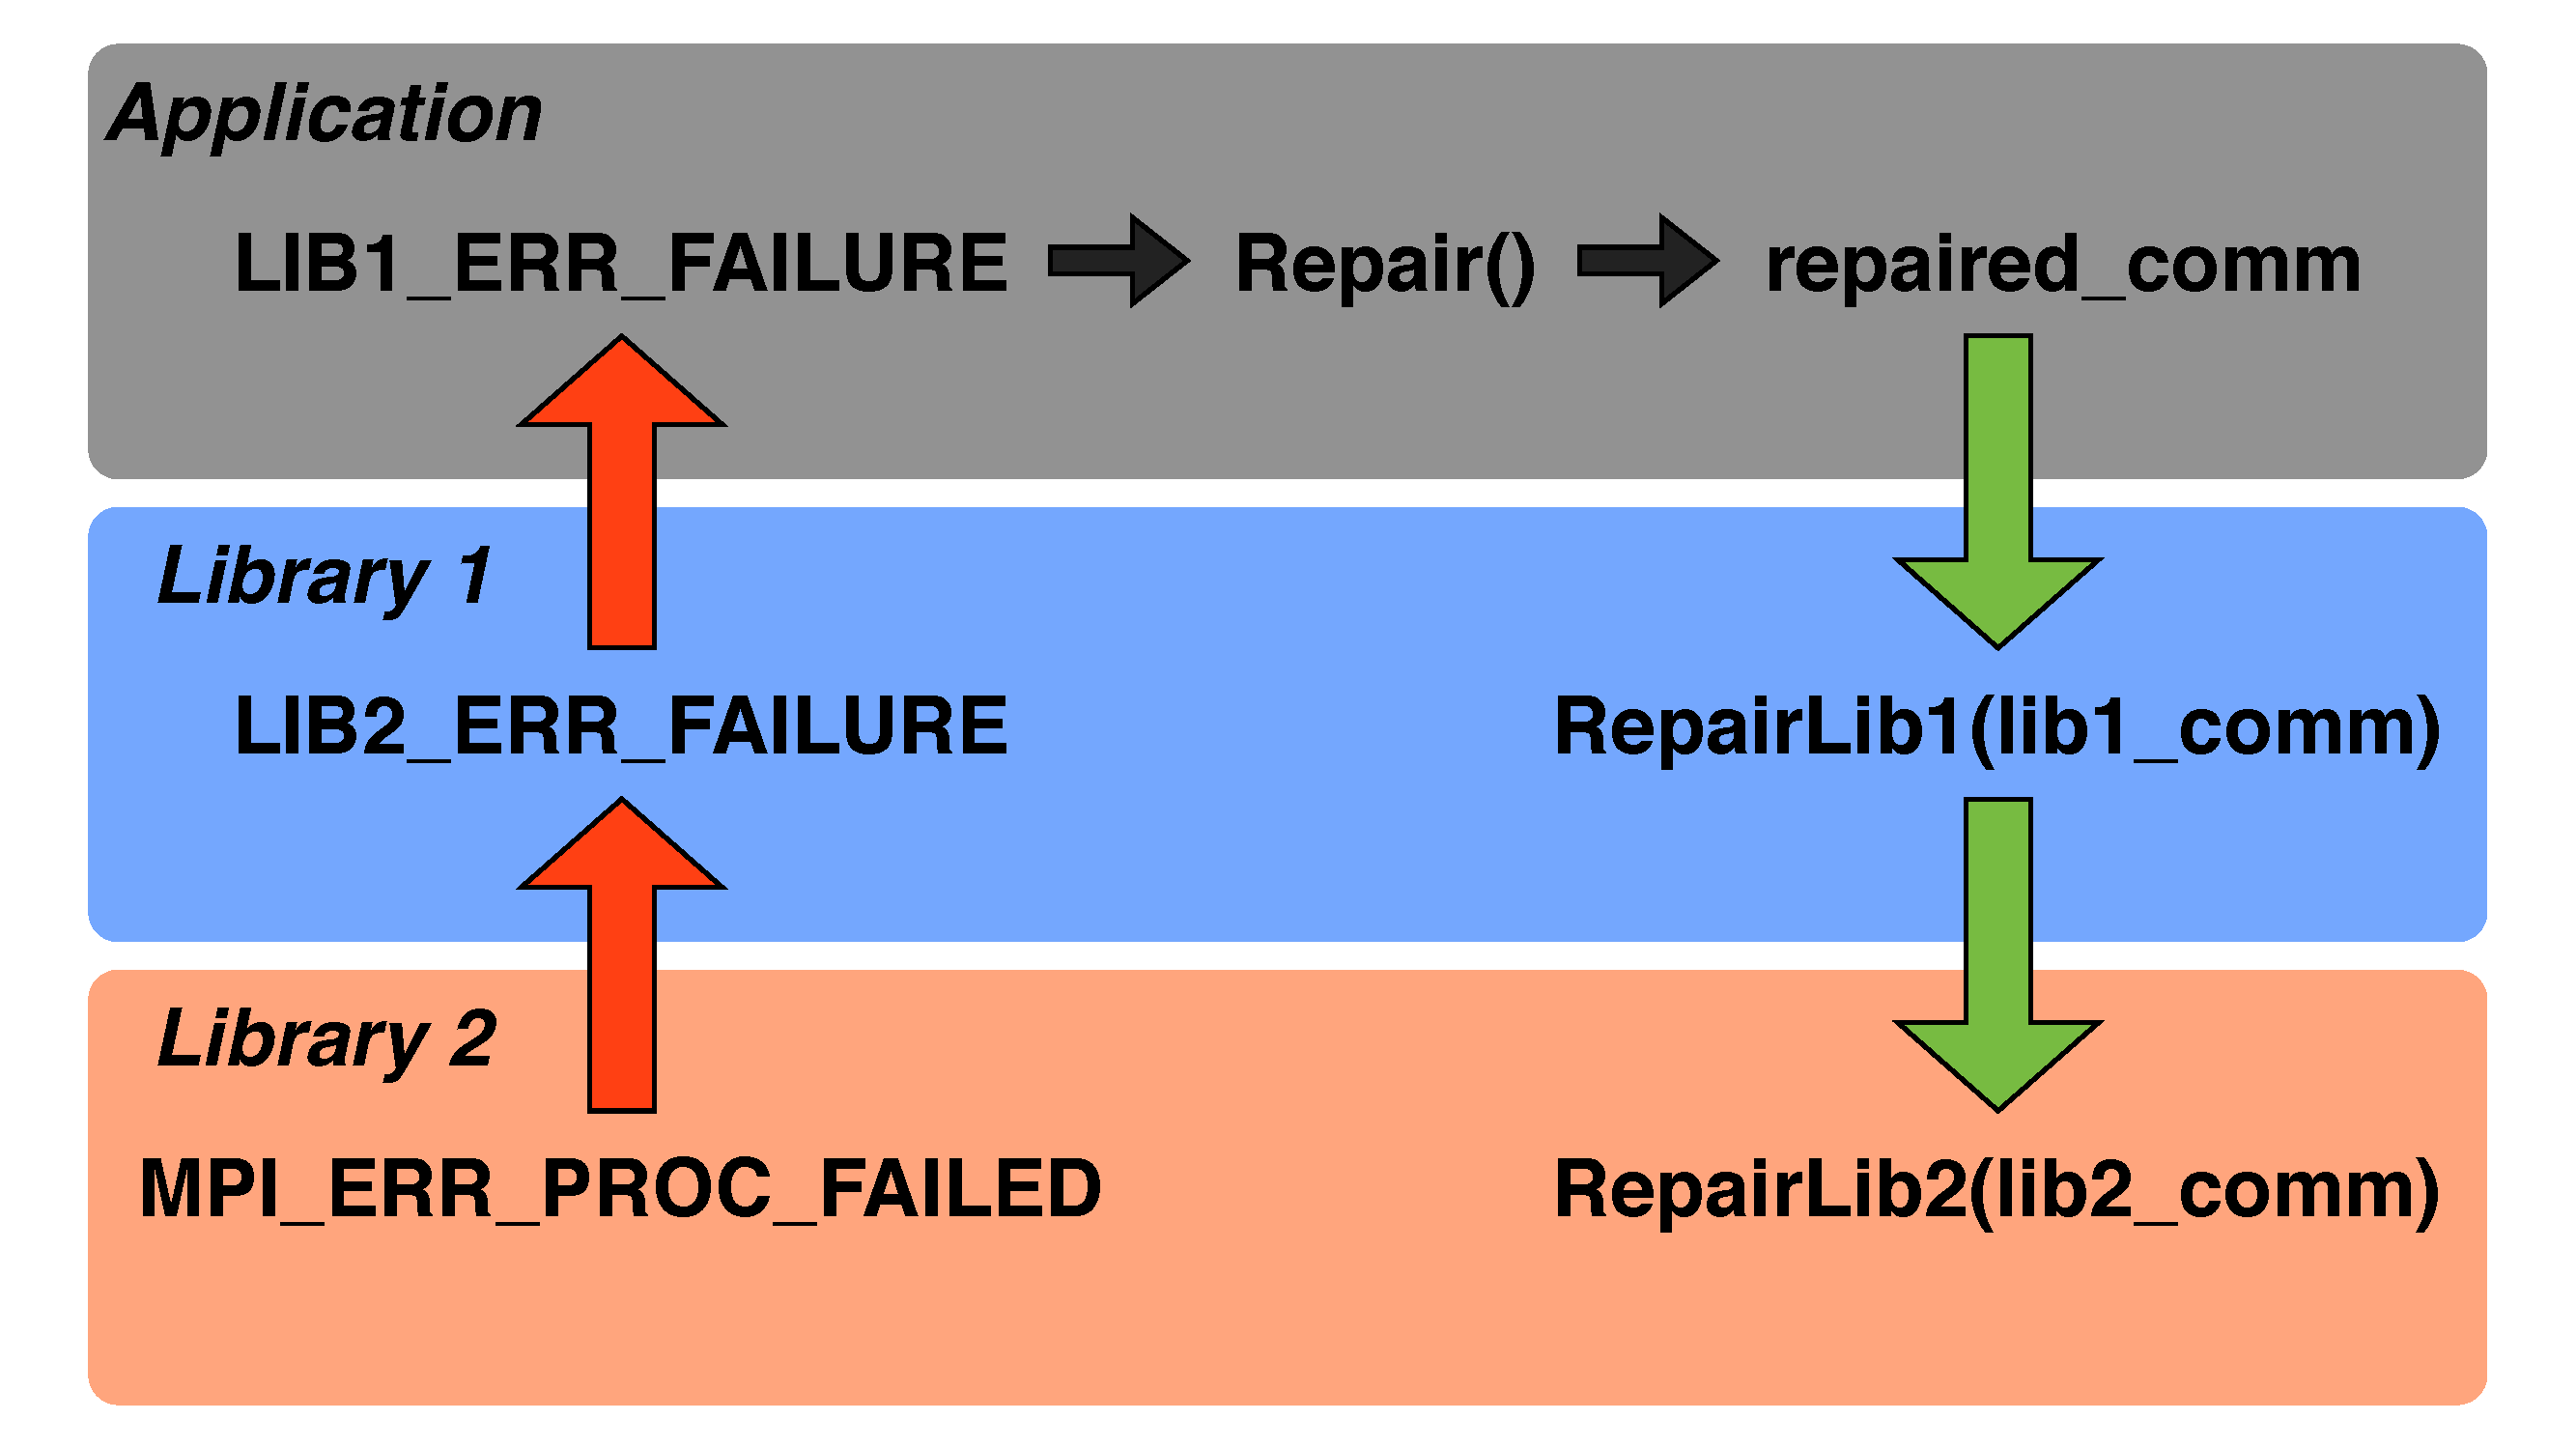
\includegraphics[width=\linewidth]{figures/libraries}
    \caption{ABFT QR and one \cof recovery on Kraken (Lustre).}    	\label{fig:apps:library-repair}	
\end{figure}

\subsubsection{Overview}

Figure~\ref{fig:apps:library-repair} demonstrates the hierarchy of libraries and 
how they should be repaired. Errors will most likely be detected by the lowest 
level library currently in use. The libraries should recursively revoke their 
communicators and return to the next level. The application should repair the 
MPI library using the appropriate measures and allow the libraries to do the same 
by calling their respective repair functions. Once all of the recovery is 
complete, the application can repeat its call to the last function it was 
attempting and execution can continue. 

Obviously, this pattern will not apply to all libraries. Some libraries 
developed to provide MPI fault tolerance directly may perform recovery 
themselves without returning to the MPI application. Some libraries may not 
include MPI calls which would necessitate recovery. However, this is a starting 
point for those interested in constructing fault tolerant MPI libraries. For a 
more complete example, see Appendix~\ref{appdx:library}.
